{\let\clearpage\relax\chapter{Przedmioty podstawowe}}

\section{APA}
\subsection{Przedstawić zasadnicze podobieństwa i różnice pomiędzy silnikami prądu stałego i prądu zmiennego. Omówić wejścia i wyjścia serwo-wzmacniaczy oraz ich rolę w układach automatyki.}

Podobieństwa w budowie:
\begin{enumerate}
    \item wirnik,
    \item uzwojenie wzbudzające (ale o różnej budowie),
    \item stojan.
\end{enumerate}


Różnice:
\begin{enumerate}
    \item Wirnik w silniku prądu zmiennego obraca się dzięki wpływowi pola magnetycznego na stojan z cewkami (pole magnetyczne wytwarzane jest przez uzwojenia w stojanie prowadzące prąd znajdujący się w różnej fazie) - dzięki indukcji uzwojenie wirnika się namagnesowuje co skutkuje ruchem obrotowym w wirującym polu magnetycznym. Silnik ten wymaga 3 różnych faz na wejściu - lub odpowiedniego modułu wewnętrznego.
    \item Wirnik w silniku prądu stałego obraca się z powodu prądu przepływającego przez uzwojenia wirnika, natomiast kierunek prądu ustalany jest przez styk szczotek wirnika ze stojanem - kierunek przepływu prądu się zmienia wraz z wykonaniem połowy obrotu. Prąd stały przechodzi przez 2 wejścia (okablowanie proste).
    \item Wirnik w silniku bezszczotkowym prądu stałego jest zbudowany z magnesu trwałego umieszczonego między trzema statorami (lub więcej) - pylonami z nawiniętymi cewkami przez które przepływa prąd. Prąd stały przechodzi przez przemiennie przez 3 z wejść (po 2 na raz) tworząc cykl (okablowanie złożone).
\end{enumerate}

Zalety silników:
\begin{enumerate}
    \item Prądu stałego: mała masa, duży moment mechaniczny, wysoka sprawność, łatwy w regulacji, wysokie obroty.
    \item Prądu stałego (bezszczotkowy): bardzo duży moment obrotowy, mała masa, bardzo dobry w regulacji, cichy, bezobsługowy, trwały, wysokie obroty.
    \item Prądu zmiennego: zasilanie z sieci, bardzo trwałe, ciche, bezobsługowe, tanie.
    \item Krokowy (impuls): bezpośrednia kontrola, cichy, trwały.
\end{enumerate}

Wady:
\begin{enumerate}
    \item Prądu stałego: zasilanie przez prostownik, drogi, wymaga konserwacji, głośny.
    \item Prądu stałego (bezszczotkowy): drogi, zasilany z przekształtnika.
    \item Prądu zmiennego: wymaga rozruchu, trudny w regulacji obrotów, ciężki, ograniczone obroty.
    \item Krokowy (impuls): zasilany z komutatora, mały moment, duża masa, kosztowny, niska sprawność (wirnik zębatkowy).
\end{enumerate}

Serwowzmacniacze są pośrednikiem między modułem generatora poleceń serwomechanizmu (komputerem), a napędem. Rolą serwowzmacniacza jest dostarczenie odpowiednio wysokiej mocy do silnika tak, aby mógł on pracować zgodnie z zadanym poleceniem. Enkoder wbudowany w serwomotor ma za zadanie odczytać wartość obrotu silnika i przesłać ją w formie sygnału zwrotnego do serwowzmacniacza, który z kolei porównuje ją z wartością sygnału polecenia. Jeżeli różnica sygnałów jest równa 0 to oznacza to, że serwomechanizm działa poprawnie.

Wejściami serwowzmacniacza są sygnał sterujący (np. z PLC) oraz sprzężenie zwrotne (z enkodera zamieszczonego w serwosilniku).

Wyjściami serwowzmacniacza są sygnał zasilający do serwosilnika oraz sygnał sprzężenia zwrotnego (opcjonalnie)


\subsection{Podać podstawową klasyfikację receptorów zwierząt ze względu na źródło bodźców, wymienić przykłady czujników stanowiących analogię dla wybranych zmysłów.}

Podstawowy podział:
\begin{enumerate}
    \item Eksteroreceptory - odbierają bodźce ze środowiska zewnętrznego:
    \begin{enumerate}
        \item telereceptory – odbierają bodźce docierające z pewnej odległości (np. receptory
wzroku, słuchu i równowagi, powonienia),
        \item kontaktoreceptory – odbierają bodźce działające bezpośrednio na receptor (np.
receptory smakowe, dotyku i nacisku, bólowe, termoreceptory).
    \end{enumerate}
    \item Interoreceptory - znajdują się wewnątrz ciała i odbierają bodźce ze środowiska wewnętrznego:
    \begin{enumerate}
        \item proprioreceptory – znajdują się w narządach ruchu (stawowe, mięśniowe); informują
o położeniu ciała oraz o lokalizacji jego części względem siebie (kinestezja),
        \item wisceroreceptory – znajdują się w narządach wewnętrznych; informują o stanie
poszczególnych narządów,
        \item angioreceptory – znajdują się w naczyniach krwionośnych; informują o stanie
środowiska w naczyniach.
    \end{enumerate}
\end{enumerate}

Przykładowe analogie:
\begin{itemize}
    \item wzrok - kamera,
    \item echolokacja - czujnik odległości,
    \item słuch - mikrofon,
    \item dotyk - czujniki kontaktu, czujniki pojemnościowe,
    \item pozycja - enkodery obrotowe, enkodery liniowe, resolver.
\end{itemize}


\subsection{Wymienić kilka wielkości fizycznych, do pomiaru których można wykorzystać ciśnieniomierze, omówić pokrótce ideę działania wybranych czujników.}

\begin{enumerate}
    \item Wysokość (m n.p.m.) - obliczana jako różnica z ciśnieniem referencyjnym, stosowany w samolotach, rakietach, balonach pogodowych, do 11km n.p.m.,
    \item Ciśnienie (Pa) - np. zmierzenie ciśnienia w oponie samochodowej,
    \item Przepływ ($\frac{\mathrm{m}^3}{\mathrm{s}}$) - zwężka Venturiego polega na zmierzeniu przepływu cieczy lub gazu na podstawie różnicy ciśnień przed i po zwężce przepływu. Wykorzystując różnicę wysokości płynu znajdującego się w łączniku rury oraz zwężenia można wyznaczyć różnicę ciśnień. Następnie znając również pola przekrojów rury i zwężenia (a dokładniej ich stosunek) oraz ciśnienie w rurze można wyznaczyć prędkość przepływu,
    \item Głębokościomierz (m) = wykorzystując wzór na ciśnienie płynu $\mathrm{P} = \rho\mathrm{g}\mathrm{h}$ można wyznaczyć wysokość słupa cieczy - czyli głębokość na jakiej się znajduje ciśnieniomierz.
\end{enumerate}

\section{MODI}
\subsection{Przedstawić założenia metody najmniejszych kwadratów (MNK). Jakie są jej ograniczenia? Jak wygląda wersja rekurencyjna MNK? Jakie są możliwe rozszerzenia?}
Założenia:
\begin{enumerate}
    \item Szacowany model ekonometryczny jest liniowy względem parametrów $\alpha_j$. 
    \item Zmienne objaśniające $X_i$ są wielkościami nielosowymi o ustalonych elementach.
    \item Rząd macierzy $X$ równy jest liczbie szacowanych parametrów, czyli $r(X) = k + 1$.
    \item Liczebność próby jest większa niż liczba szacowanych parametrów, tzn. $n \geq k+1$.
    \item Nie występuje zjawisko współliniowości pomiędzy zmiennymi objaśniającymi.
    \item Wartość oczekiwana składnika losowego jest równa zero: $\forall_t E(\epsilon _t) = 0$.
    \item Składnik losowy ma stałą skończoną wariancję  $\forall_t D^2(\epsilon _t) = \sigma^2$.
    \item Nie występuje zjawisko autokorelacji składnika losowego, czyli zależności składnika losowego w różnych jednostkach czasu  $\forall_{t\neq s} cov(\epsilon _t, \epsilon_s) = 0$.
    \item Składnik losowy ma n-wymiarowy rozkład normalny: $\epsilon _t : N(0,\sigma^2)$ dla t=1,2,…,n.
\end{enumerate}

Objaśnienia:

\textbf{1.} Ogólnie, w modelu typowo liniowym główną rolę odgrywa suma iloczynów typu  " $+ a_iX_i +$" . To znaczy, że zarówno parametry, jak i zmienne powinny być jednocześnie w pierwszych potęgach, oraz zmienna objaśniana Y powinna być kombinacją liniową zmiennych objaśniających i różnych parametrów.

Stąd taki model można zapisać w postaci macierzowej: $Y = X\alpha + \epsilon$.

Wektor epsilon grupuje składniki losowe które są z definicji nieobserwowalne, postulujemy ich istnienie, by wyjaśnić wszelkie rozbieżności między teoretycznymi wartościami zmiennej objaśnianej a wartościami zaobserwowanymi. 

W praktyce liczymy się z tym, że Z1 nie jest idealnie spełnione.

\textbf{2.} Zmienne objaśniające są nielosowe. Ich wartości traktowane są jako stałe w powtarzających się próbach.

\textbf{3.} Chodzi tu o niezależność pomiędzy zmiennymi objaśniającymi.

Założenia te zapewnia, że estymator można wyznaczyć w sposób jednoznaczny.

Z założenia 3 wynika od razu założenie 4 i założenie 5. Dlatego czasami wypisanie tych założeń osobno jest pomijane.

\textbf{4.} Liczba obserwacji n powinna być większa od liczby szacowanych parametrów (zmiennych objaśniających).

\textbf{5.} Zmienne objaśniające nie mogą być współliniowe, tzn. wektory obserwacji zmiennych objaśniających (kolumny macierzy X) powinny być liniowo niezależne.

Jeżeli istnieje liniowość to skoro widzimy, że coś się dzieje, to wypadałoby dojść do tego, co tam się kryje. Najprawdopodobniej w wartościach składnika losowego, w przypadku wystąpienia jego autokorelacji, zawarty jest jakiś czynnik mający spory wpływ na kształtowanie się zmiennej objaśnianej. Czynnik, którego nie wzięliśmy pod uwagę rozważając to, co może wpływać na badane przez nas zagadnienie.

\textbf{6.} Wartości oczekiwane składników losowych są równe zeru. Oznacza to, że zakłócenia reprezentowane przez składniki losowe mają tendencję do wzajemnej redukcji.

\textbf{7.} Wariancje składników losowych $\epsilon_t$ są stałe. Jest to tak zwana własność homoskedastyczności.

Macierz wariancji i kowariancji pomiędzy składnikami resztowymi jest postaci: $D^2 = \sigma^2\textbf{I}$.

Założenie to zapewnia, że wartość wariancji zakłóceń nie zależy od numeru obserwacji.

\textbf{8.} Składniki losowe $\epsilon_t$ i $\epsilon_s$ są od siebie niezależne. Nie występuje tzw. autokorelacja składników losowych.

Oznacza to liniową zależność pomiędzy resztami modelu odległymi od siebie o “k” okresów. Dotyczy to modeli dynamicznych.

Jej występowanie oznacza, że pominięto w modelu jedną z istotnych zmiennych objaśniających lub przyjęto niewłaściwą postać modelu.

\textbf{9.} Każdy ze składników losowych $\epsilon_t$ ma rozkład normalny.

Założenie to dotyczące normalności rozkładu składnika losowego ma znaczenie przy wnioskowaniu statystycznym.

\textbf{Ograniczenia}

Metoda najmniejszych kwadratów jest mało odporna na elementy odstające, czyli nieliczne obserwacje różniące się znacząco od pozostałych. Takie obserwacje przyciągają do siebie linię trendu, co może być niepożądane w niektórych zastosowaniach. Niemniej jednak o ile odstające informacje nie są wynikiem błędnego pomiaru, nie powinny one być usuwane z modelu, ponieważ prowadziłoby to do błędnej estymacji parametrów modelu oraz do niedoszacowania zmienności zmiennej zależnej niewyjaśnionej przez model, a zatem wnioskowanie statystyczne na podstawie takiego modelu byłoby nieprawidłowe. Jeśli wpływ obserwacji odstających jest niepożądany, należy rozważyć zastosowanie innych metod regresji (np. regresji odpornej).

\begin{description}
    \item[Uogólniona MNK] - Pozwala ona na uwzględnienie braku sferyczności błędów losowych. 
    \item[Ważona MNK] - Jeżeli macierz wariancji-kowariancji jest znana i jest ona macierzą diagonalną o elementach $var{[E_i|x_i]} = \sigma^2\omega_i$ to przypisujemy poszczególnym obserwacjom wagi.
    \item[Regresja grzbietowa] - Redukcja wariancji modelu kosztem jego obciążenia (zmniejsza MSE estymatorów w stosunku do MNK). Umożliwia estymację przy wysokiej współliniowości.
    \item[Całkowite NK] - Zakładamy, że błąd dotyczy wyjścia oraz pomiarów w wektorze regresji.
    \item[Rozszerzone NK] - Podobnie jak regresja grzbietowa, rozszerza metodę MNK na modele, w których zakłócenia są ze sobą skorelowane. Ponieważ jednak zakłócenia nie są mierzalne to model regresji jest budowany przez aproksymację zakłóceń obliczając błąd predykcji - m.in. modele ARMAX.
\end{description}


\subsection{Jakie są możliwe sygnały identyfikacyjne? Kiedy je stosujemy? Jakie mają ograniczenia? }
\begin{itemize}
    \item Impuls
    \item Skok jednostkowy - tylko do obiektów o nieskomplikowanej dynamice (1, 2-inercyjne z opóźnieniem).
    \item Sygnał binarny
    \item Sygnał Gaussa
    \item Pseudolosowy sygnał binarny - rodzaj białego szumu (pobudza szeroki zakres częstotliwości).
    \item Sinusoida - suma kilku sygnałów sinusoidalnych o różnych częstotliwościach. Do identyfikacji charakterystyk Bodego (amplitudowa i fazowa), Nyquista (amplitudowo-fazowa).
\end{itemize}

Przy wyborze sygnału należy zwrócić uwagę na:
\begin{itemize}
    \item Możliwą do realizacji dynamikę wejścia (urządzenie wykonawcze)
    \item Typ identyfikowanego modelu (liniowy - skok jednostkowy, nieliniowy - sinusoida)
    \item Jakie mamy praktyczne możliwości oddziaływania na proces (pozwolenia od operatorów)
\end{itemize}

\subsection{Przedstawić różne postacie modeli regresyjnych od AR aż do Boxa-Jenkinsa oraz modele z całkowaniem.}
\label{pyt:6}
\textbf{Ogólna postać modelu regresyjnego:}\mbox{}\\
$Y=f(X,\beta)+\varepsilon$


S - gdy w badanym procesie występuje sezonowość (m)

AR(p) – autoregresja (rząd opóźnienia p)

I(d) – stopień integracji szeregu (krotność różnicowania d)

MA(q) – średnia ruchoma (rząd opóźnienia q)

ARX(r) - model autoregresywny z zewnętrznym wejściem

\textbf{MA} Charakterystyczna dla tego modelu jest propagacja losowych zaburzeń do przyszłych wartości szeregów czasowych. Interpretacja: Zadanie impulsu wejściowego sprawia, że wyjście modelu gwałtownie rośnie, a następnie powoli opada - rozłożenie średniej w czasie.

MA jest z definicji zależne od wejść stochastycznych (zakłóceń).

\textbf{AR} Charakterystyczna dla tego modelu jest liniowa zależność wyjścia od poprzednich jej wartości. Interpretacja: Wyjście obiektu jest jak filtr o nieskończonej odpowiedzi ze wszystkimi biegunami stabilnymi.

AR jest zależne od wyjść.

Modele AR i MA są względem siebie dualne - każde AR o skończonym rzędzie można opisać jako MA o nieskończonym rzędzie.

\textbf{ARX} Wykorzystywany w modelach, w których zakłócenia pojawiają się wcześnie. Sygnał stochastyczny (zakłóceń) oraz deterministyczny (sterowania) przechodzą razem przez blok 1/A - oznacza to, że dynamika odpowiedzi układu dla obu tych sygnałów wejściowych jest taka sama.

\textbf{OE} Jeżeli zakłócenia pojawiają się późno to lepiej zastosować model OE (output-error) - w tym modelu sygnał stochastyczny nie przechodzi przez blok 1/A, czyli przez bloki B oraz 1/A przechodzi tylko sygnał deterministyczny.

\textbf{Box-Jenkins} Jest to kompletny model z zakłóceniami modelowanymi oddzielnie od dynamiki systemu. Również stosowany najlepiej, gdy zakłócenia pojawiają się późno w systemie. Jest to połączenie modeli ARMA oraz OE.

Wygląd sygnału, a model:
\begin{description}
    \item[AR] - Wykładniczy, opadający do zera lub oscylacje pozytywno-negatywne, również opadające do zera.
    \item[MA] - Jeden lub więcej nagłych skoków, w pozostałości praktycznie zero.
    \item[ARMA] - Opadający do zera, po kilku opóźnieniach.
    \item[SAR] - Sezonowy model stosowany w przypadku, gdy pojawia się wiele wysokich skoków wyjścia w równych interwałach.
    \item[Brak] - Nie opada do zera lub wszystko jest zerem lub blisko zera.
\end{description}


\begin{figure}[!h]
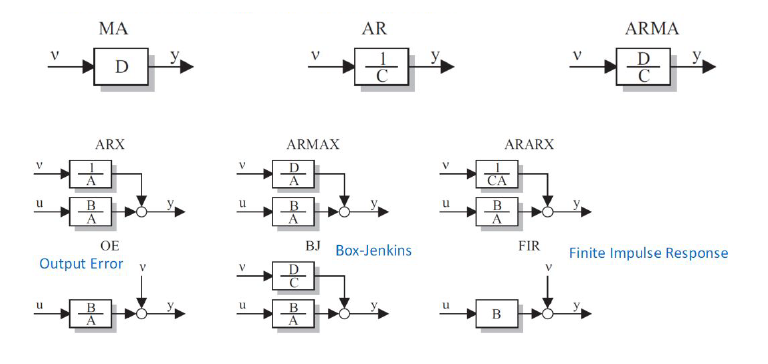
\includegraphics[width=\linewidth]{fig/Modele.png}
\end{figure}


\textbf{Modele z całkowaniem}

Zmieniając zmienne z absolutnych na przyrostowe uzyskamy model z całkowaniem (np. ARIMA albo ARIMAX). Jest on użyteczny w przypadku, gdy model obiektu okazuje się być niestacjonarny, bo pozwala usunąć trend.

\textbf{Identyfikacja}

Wszystkie powyższe modele są liniowe względem parametrów, więc można je przedstawić w postaci typowej dla regresji liniowej i dobrać wektor parametrów metodą najmniejszych kwadratów. Nie zawsze jest to jednak możliwe – przeszłe wartości zakłóceń są nieobserwowalne, w związku z czym w przypadku modeli zawierających człon MA konieczne jest stosowanie metod iteracyjnych (w których wartość przeszłych zakłóceń estymuje się na podstawie błędu predykcji). Zakłócenie z danej chwili (występujące we wszystkich modelach) zakłada się, że jest zerowe (to najlepszy możliwy strzał, ponieważ taka jest wartość oczekiwana wejścia stochastycznego. Nie możemy wykorzystać wartości wyliczonej na podstawie poprzedniego kroku ponieważ zakładamy, że każda kolejna wartość na wejściu stochastycznym stanowi niezależną zmienną losową, innymi słowy – nie ma żadnego związku z poprzednimi wartościami). 

Podczas identyfikacji istotnym czynnikiem jest korelacja sygnałów. Np. w przypadku MNK zastosowanej do modelu ARX błąd doboru parametrów dąży do wielkości zależnej od wartości oczekiwanej z iloczynu wejścia deterministycznego i stochastycznego. Wartość ta jest zerowa tylko wtedy, jeśli zakłócenia stanowią szum biały.

Jeżeli jednak aktualna wartość zakłóceń jest skorelowana z którąkolwiek zmienną braną pod uwagę w regresji liniowej (czyli np. z poprzednimi wartościami zakłóceń albo wartościami sygnału deterministycznego), wówczas MNK daje niedokładne rezultaty i należy zastosować metodę zmiennej instrumentalnej (pytanie 31) albo zmienić model na bardziej adekwatny np. nieliniowy względem parametrów (wtedy zastosować metodę błędu predykcji). Zazwyczaj zależy nam na zidentyfikowaniu wektorów A i B. Wektory C i D na schemacie oznaczają wtedy, że zdajemy sobie sprawę, że szum jest kolorowy.

\section{PODA}
\subsection{Sposoby opisu ciągłych liniowych układów dynamicznych. Omówić równania stanu, transmitancje, charakterystyki częstotliwościowe i odpowiedzi skokowe.}
\textbf{Równanie dynamiki}

Równanie różniczkowe wyrażające zależność pomiędzy sygnałem wejściowym i wyjściowym nazywa się równaniem dynamiki.

\begin{equation}
    a_n\frac{d^ny}{dt^n} + a_{n-1}\frac{d^{n-1}y}{dt^{n-1}} + ... + a_0y = b_m\frac{d^mx}{dt^m} + b_{n-1}\frac{d^{m-1}x}{dt^{m-1}} + ... + b_0x
\end{equation}

\textbf{Równania stanu}

Z równania dynamiki można następnie wyznaczyć równania różnicowe stanu.

\begin{equation}
    \begin{split}
    \dot{x}(t) &= Ax(t)+Bu(t)  \\
    y(t) &= Cx(t) + Du(t)
    \end{split}
\end{equation}


\textbf{Transmitancje}

Modele opisane liniowymi równaniami lub układami równań różniczkowych można przekształcić do algebraicznych modeli operatorowych. Najpopularniejsze z nich to transmitancje, oparte na przekształceniach całkowych Laplace’a (L) i Fourier’a (F). Zastosowanie całkowego operatora Laplace’a L powoduje, że funkcje zależne od czasu zostają przekształcone w funkcje zmiennej s (transformaty funkcji), a zamiast pochodnych funkcji występują potęgi zmiennej s, czyli funkcje algebraiczne.


\begin{equation}
    G(s) = \frac{Y(s)}{U(s)}
\end{equation}

Transmitancja G(s) liniowego, stacjonarnego układu dynamicznego jest równa ilorazowi transformat Laplace’a, odpowiednio, przebiegu wyjścia i wejścia, przy zerowych warunkach początkowych.


\textbf{Portrety fazowe}

Jest to rodzina trajektorii w układzie współrzędnych [x, x'], przedstawiających zachowanie obiektu obserwowane przy stałym wymuszeniu ale dla różnych warunków początkowych, które są wówczas jedyną przyczyną zmian obserwowanych w układzie. Jest to graficzny sposób zobrazowania własności dynamicznych obiektów 1. lub 2. rzędu liniowych i nieliniowych. Portrety fazowe najłatwiej jest uzyskać metodami symulacyjnymi na podstawie równań różniczkowych. Ilość trajektorii koniecznych do odtworzenia portretu można znacznie ograniczyć ze względu na jedną z podstawowych własności – trajektorie nie przecinają się ponieważ badane są układy deterministyczne. 

\textbf{Charakterystyki częstotliwościowe}

Wyróżnia się dwa rodzaje charakterystyk częstotliwościowych. Bodego i Nyquista.

Zapewnienie stabilnego działania jest podstawowym wymaganiem, jakie stawiamy układowi automatycznej regulacji. Jednym z kryteriów badania stabilności jest kryterium Nyquista, które służy do oceny stabilności liniowego zamkniętego układu regulacji na podstawie znajomości charakterystyki częstotliwościowej układu otwartego. Badając otwarty układ regulacji możliwe są dwie sytuacje:
\begin{itemize}
    \item otwarty układ regulacji jest stabilny,
    \item otwarty układ regulacji jest niestabilny.
\end{itemize}
Jednocześnie do analizy stabilności układów regulacji w oparciu o kryterium Nyquista można wykorzystać dla rodzaje charakterystyk częstotliwościowych:
\begin{itemize}
    \item amplitudowo – fazowe (charakterystyki Nyquista),
    \item logarytmiczne (charakterystyki Bode’a). 
\end{itemize}

\textbf{Charakterystyka Bodego} obrazuje logarytmiczną zależność amplitudy i fazy od częstotliwości. Składa się z dwóch wykresów: charakterystyki amplitudowej i charakterystyki fazowej.

Aby oddać zmiany zachodzące przy przejściu sygnału przez system wyznacza się dwie charakterystyki: jedną dla zmian amplitudy, a drugą dla przesunięcia w fazie. W ten sposób możemy zobaczyć, jak, dla określonych częstotliwości sygnału wejściowego zmienia się amplituda oraz przesunięcie fazy pomiędzy sygnałem wyjściowym i wejściowym. Skala częstotliwości przedstawiana jest na wykresach w postaci logarytmicznej, skala amplitudy w decybelach, a skala przesunięcia fazowego w kątach lub w radianach.

\begin{figure}[!h]
\centering
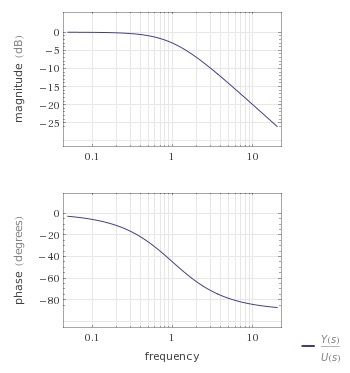
\includegraphics[width=0.5\linewidth]{fig/Bode.png}
\end{figure}

Z wykresów widać, że dla bardzo niskich częstotliwości sygnału wejściowego możemy założyć, że charakterystyka amplitudowa jest tak mała, że można ją pominąć (dla tego zakresu częstotliwości amplituda sygnału wyjściowego będzie równa amplitudzie sygnału wejściowego). Natomiast dla częstotliwości wyższych amplituda maleje, co oznacza, że po przekroczeniu pewnej częstotliwości sygnału wejściowego, sygnał wyjściowy będzie coraz mocniej tłumiony.


\textbf{Kryterium Nyquista}

W zależności od położenia punktów przecięcia charakterystyki amplitudowo – fazowej (charakterystyki Nyquista) z osią rzeczywistą, względem punktu krytycznego (– 1, j0), charakterystyka ta dzieli się na dwa rodzaje:
\begin{itemize}
    \item charakterystyka I rodzaju – wszystkie punkty przecięcia leżą na prawo od punktu krytycznego (– 1, j0),
    \item charakterystyka II rodzaju – punkty przecięcia leżą po obu stronach punktu krytycznego (– 1, j0). 
\end{itemize}

Jeżeli liniowy otwarty układ regulacji jest stabilny i jego charakterystyka amplitudowo – fazowa (charakterystyka Nyquista) dla pulsacji  $\omega\in (0, \infty)$ nie obejmuje punktu $(-1,j_0)$, to układ ten po zamknięciu będzie stabilny. 

Liniowy zamknięty układ regulacji jest stabilny, jeżeli punkt (-1, j0) znajduje się w obszarze leżącym po lewej stronie charakterystyki amplitudowo – fazowej (charakterystyki Nyquista)  $G(\omega)$, przesuwając się w kierunku rosnących pulsacji $\omega$. 

\textbf{Odpowiedzi skokowe}

Reakcja układu na podanie wymuszenia w postaci skoku jednostkowego na wejście układu.
Odpowiedź skokowa ilustruje dynamikę/wyjście/odpowiedź układu. Odpowiedź skokowa
jest to wykres w przestrzeni czasu. Z odpowiedzi skokowej można odczytać takie informacje
jak:
\begin{enumerate}
    \item czy układ się stabilizuje, czy oscyluje, czy się rozbiega,
    \item jak długo czas się stabilizuje,
    \item czy układ ma opóźnienie,
    \item wzmocnienie układu,
    \item przeregulowanie.
\end{enumerate}

\subsection{Omówić sprzężenie zwrotne i jego wpływ na dokładność, odporność na błędy i zakłócenia oraz stabilność układu sterowania. Przedstawić warunki podtrzymania drgań oraz kryterium Nyquista dla obiektu stabilnego. Zdefiniować pojęcia zapasu fazy i modułu.}

\textbf{Sprzężenie zwrotne} jest to połączenie elementów, w którym sygnał wyjściowy z bloku w torze głównym oddziałuje wstecznie na sygnał wejściowy tego bloku. Sprzężenie zwrotne poprawia skuteczność sterowania. Zamknięta ujemna pętla sprzężenia zwrotnego ma właściwości stabilizujące i linearyzujące. Układ zamknięty jest mniej czuły na zmiany wzmocnienia statycznego układu, powodując zmniejszenie uchybów statycznych. Zbyt duże wzmocnienie może prowadzić jednak do niestabilności. Sprzężenie zwrotne poprawia również parametry jakościowe odpowiedzi skokowej i dobrze sprawdza się w przypadku tłumienia nieznanych zakłóceń.

\textbf{Dodatnie sprzężenie zwrotne}:
\begin{description}
    \item[-] wzrost zniekształceń
    \item[+] przy wzroście współczynnika sprzężenia w układzie wystąpi generacja drgań, a nieskończone wzmocnienie oznacza, że generator sam dostarcza na wejście sygnał podtrzymujący drgania. Sygnał wyjściowy zostanie ograniczony do pewnej wartości określonej przez układ - nie może być ona wyższa od napięcia zasilającego wzmacniacz.
\end{description}

Dodatnie sprzężenie zwrotne jest podstawą działania generatorów, przy czym warunki generacji można wyrazić następująco: układ działa jak generator, gdy sprzężenie zwrotne jest dodatnie i dostatecznie silne ($\beta\cdot{}K=1$, K - współczynnik pętli głównej, a $\beta$ sprzężenia) , aby podtrzymać drgania.

Jeżeli $\beta\cdot{}K<1$ to w układzie następuje tylko wzrost wzmocnienia.

\textbf{Ujemne sprzężenie zwrotne}:
\begin{description}
    \item[+] poprawia stabilność wzmocnienia (układ jest mniej wrażliwy na np. wahania napięć zasilających i temperatury),
    \item[+] zmniejszają się szumy i zniekształcenia (liniowe i nieliniowe),
    \item[+] zwiększa się górna częstotliwość graniczna (czyli ulega polepszeniu pasmo przenoszenia wzmacniacza),
    \item[+] możliwe jest kształtowanie charakterystyki częstotliwościowej,
    \item[+] możliwa jest modyfikacja impedancji wejściowej i wyjściowej.
\end{description}

\textbf{W celu podtrzymania drgań} w generatorze wymagane jest spełnienie niezależnie dwóch warunków:
\begin{enumerate}
    \item fazy - musi zachodzić zgodność sygnałów na wejściu i wyjściu wzmacniacza: $\phi_{we}+\phi_{wy} = n\times{}360\deg$,
    \item amplitudy - $\beta{}\cdot{}K=1$.
\end{enumerate}

\textbf{Kryterium Nyquista}
\begin{itemize}
    \item odnosi się do relacji układ otwarty -> układ zamknięty pętlą ujemnego sprzężenia zwrotnego o jednostkowym wzmocnieniu,
    \item pozwala badać stabilność układu zamkniętego na podstawie przebiegu charakterystyki częstotliwościowej układu otwartego, którą można wyznaczyć analitycznie lub doświadczalnie.
\end{itemize}

Jeżeli charakterystyka amp-faz otwartego układu regulacji automatycznej dla częstotliwości $\omega$ nie obejmuje punktu $(-1,j_0)$ to wtedy i tylko wtedy po zamknięciu będzie on równie stabilny.

Układ zamknięty jest stabilny tylko wtedy, gdy punkt $(-1,j_0)$ znajduje się w obszarze leżącym po lewej stronie charakterystyki, idąc od początku w stronę rosnących częstotliwości $\omega$ -> reguła lewej strony.

Jeżeli hodograf (charakterystyka fazowa Nyquista) przehodzi przez punkt stabilności to układ jest na granicy stabilności.

\textbf{Zapas modułu i fazy} to wielkości charakteryzujące od strony ilościowej stabilność układu zamkniętego.

Zapas modułu: $a = \frac{1}{\left|G_0(j\omega_\phi)\right|}$

Zapas fazy: $\Delta\phi = 180\deg + \mathrm{arg}G_0(j\omega_g)(\deg)$

Pomnożenie wzmocnienia przez zapas modułu powoduje, że układ zamknięty znajduje się na granicy stabilności.

\clearpage
Zapas modułu i fazy na wykresie Nyquista:
\begin{figure}[!h]
\centering
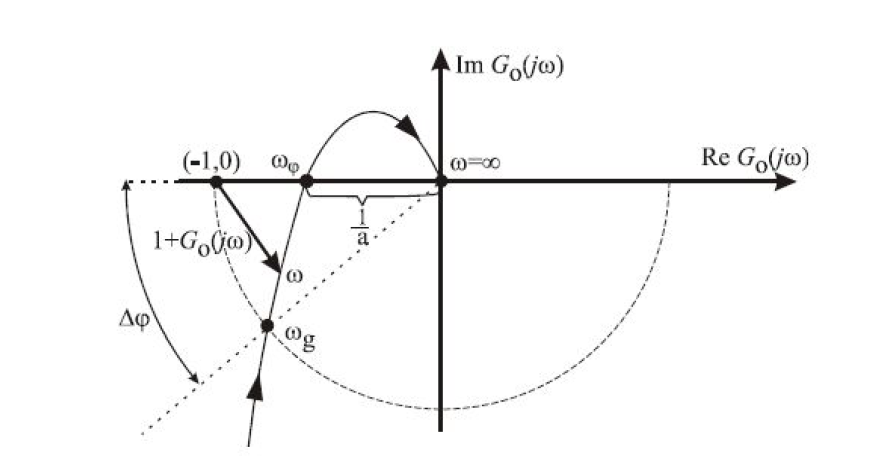
\includegraphics[width=0.7\linewidth]{fig/Zapasy amp i fazy.png}
\end{figure}

\textbf{Zapas stabilności} stanowi zabezpieczenie, że gdy przy pewnych zmianach parametrów układu, które mogą zachodzić podczas pracy lub z upływem czasu, to mogą występować przesunięcia charakterystyk w niekorzystnym kierunku, a układ dalej pozostaje stabilny.


\subsection{Omówić wybrane metody projektowania prostych układów regulacji: dla serwomechanizmów (obiektów minimalnofazowych) oraz dla regulacji przemysłowej (modelowanie obiektów, struktury i podstawowe metody doboru nastaw regulatorów PID).}

\textbf{Wymagania projektowania układu regulacji}
\begin{enumerate}
    \item Układ zamknięty musi być asymptotycznie stabilny, przy czym potrzebne jest zapewnienie odpowiednich zabezpieczeń (np. zapasów) stabilności.
    \item Sygnał y(t) powinien jak najlepiej (jak najdokładniej) nadążać za przebiegiem wartości zadanej.
    \item Należy w jak największym możliwym stopniu wyeliminować wpływ zakłóceń.
    \item Przebiegi przejściowe będące skutkiem różnych od zera warunków początkowych, bądź wynikające z załączenia układu lub zmiany wartości zadanej - na przykład skoku - powinny mieć odpowiedni kształt.
\end{enumerate}

Projektowanie jest sztuką kompromisu między tymi wymaganiami.

\textbf{Projektowanie serwomechanizmu} - dany jest obiekt minimalnofazowy (bez opóźnienia i zer w prawej półpłaszczyźnie), ponadto zakładamy, że istotne jest uzyskanie odpowiedniej dokładności odtwarzania sygnałów zmiennych w czasie, skoncentrowanych w zadanym paśmie roboczym oraz zapewnienie tłumień pomiarowych, wpływ zakłóceń procesowych jest w zasadzie pomijalny.

\textbf{Projektowanie układu regulacji przemysłowej} - dany jest obiekt minimalnofazowy lub częściej, nieminimalnofazowy. Ponadto istotne jest uzyskanie odpowiednio małego (bądź zerowego) uchybu w stanie ustalonym oraz możliwie najlepsze tłumienie zakłóceń procesowych. Wpływ zakłóceń pomiarowych jest najczęściej pomijalnie mały.

\textbf{Projektowanie serwomechanizmu}

Założenia:
\begin{itemize}
    \item pomijamy wpływ zakłóceń obiektowych z(t),
    \item przyjmujemy, że sygnały określające wartość zadaną yzad(t) mają składowe sinusoidalne o pulsacjach dodatnich ograniczonych poprzez wartość $\omega_r$ - pulsacje robocze,
    \item sygnały określające zakłócenia pomiarowe v(t) mają także przebiegi sinusoidalne,
    \item transmitancja obiektu G(s) ma postać $G(s) = \frac{L(s)}{s^2M(s)}$. Ponadto nie ma ona zer i biegunów w prawej półpłaszczyźnie, tzn. zarówno wielomian licznikowy L(s) nie ma pierwiastków (zer transmitacyjnych) w prawej półpłaszczyźnie, jak i wielomian M(s) nie ma pierwiastków (biegunów transmitancji) w prawej półpłaszczyźnie.
\end{itemize}

Sensowny układ sterowania da się zaprojektować wówczas, gdy $\omega_v > \omega_r$, tzn. wtedy, gdy występuje rozdzielczość pasm sygnałów zakłócających i sygnałów zadanych. Gdy te pasma na siebie wyraźnie nachodzą, konieczne jest poprawienie urządzeń pomiarowych. Trzeba je tak zmienić, aby pasmo zakłóceń nie pokrywało się z pasmem pulsacji roboczych.

Standardowe wymagania projektowe:
\begin{description}
    \item[Stabilność] - bezwzględnie wymagane uzyskanie asymptotycznej stabilności oraz zapewnienie odpowiednich zapasów modułu (6dB) i fazy (45deg).
    \item[Dokładność] - może być wyrażona jako wymaganie dokładności nadążania. Może temu towarzyszyć także wymaganie zapewnienia zerowego uchybu w stanie ustalonym.
    \item[Tłumienie zakłóceń pomiarowych] - należy zapewnić jak najlepsze tłumienie zakłóceń v(t) dla $\omega \geq \omega_v$.
\end{description}

Projektowanie w takiej sytuacji polega na kształtowaniu przebiegu logarytmicznej charakterystyki amplitudowej przy pomocy odpowiedniego doboru transmitancji regulatora R(s).

Przebieg charakterystyki amplitudowej układu otwartego:
\begin{enumerate}
    \item Logarytmiczna charakterystyka modułu układu otwartego musi przechodzić ponad tzw. prostokątem dokładności o wysokości $20log\frac{1}{d}$, sięgającym na osi pulsacji do wartości $\omega_r$, po to, by dla pulsacji $\omega \geq \omega_v$ spełnione było wymaganie $|G(j\omega)R(j\omega)|\geq \frac{1}{d}$.
    \item Następnie możliwie jak najbliżej wartości $\omega$ równej $\omega_r$ nachylenie charakterystyki powinno osiągać wartość -2. Wynika to z tego, aby wzmocnienie toru otwartego malało dla pulsacji wyższych niż $\omega_r$ możliwie szybko w celu tłumienia zakłóceń pomiarowych.
    \item W celu zapewnienia asymptotycznej stabilności układu zamkniętego w okolicy pulsacji odcięcia amplitudy $\omega_g$, gdzie $20log|G(j\omega)R(j\omega)| = 0$, należy zapewnić nachylenie charakterystyki modułu równe -1, przez dekadę. Nachylenie równe -1 musimy utrzymać na odcinku odpowiadającym mniej więcej jednej dekadzie, tj. od $\omega = \omega_a$ do $\omega=10\omega_a$ oraz $20log|G(j\omega)R(j\omega)| \approx 8 \div 10dB$.
    \item Po osiągnięciu przez pulsację wartości równej $10\omega_a$ nachylenie charakterystyki modułu powinno znowu przyjąć wartość równą -2, aby nadal szybko zmniejszać wzmocnienie toru otwartego i tym samym zapewnić jak najlepsze tłumienie zakłóceń charakteryzujących się wysokimi częstotliwościami.
\end{enumerate}

\textbf{Regulacja przemysłowa}

Układ regulacji przemysłowej - układy regulacji takich wielkości jak temperatura, ciśnienie, przepływ, poziom itp. występujące przede wszystkim w zakładach przemysłowych, energetycznych itp. W odróżnieniu od serwomechanizmów, gdzie wielkość regulowana ma charakter przesunięcia liniowego lub kątowego.

Cechy zadań regulacji przemysłowej:
\begin{itemize}
    \item Sygnał wielkości zadanej jest najczęściej stały w dłuższych odcinkach czasu (tzw. zadanie regulacji stałowartościowej lub zadanie stabilizacji), o wartości zmienianej bardzo rzadko. Sygnał wartości zadanej może być też zmieniany w czasie, np. w z góry zaprogramowany sposób (tzw. regulacja programowa), czy też np. jako sygnał wyjściowy regulatora nadrzędnego zmienny w sposób wynikający z bieżącego działania tego regulatora (regulacja nadążna).
    \item Z reguły zadanie tłumienia zakłóceń jest najistotniejsze.
    \item Standardem jest stosowanie regulatora PID, przy czym najczęściej dysponujemy jedynie bardzo uproszczonym modelem obiektu utworzonym specjalnie dla zadania doboru nastaw regulatora.
\end{itemize}

Regulator PID:
\begin{description}
    \item[+] prosta struktura
    \item[+] realizacja podstawowych celów: tłumienie zakłóceń przy poszerzaniu pas przenoszenia skutkujące dobrą szybkością regulacji również w zadaniu nadążania
    \item[+] zerowe uchyby regulacji w stanach ustalonych - dzięki całkowaniu
    \item[+] dodatkowe dodatnie przesunięcie fazowe w zakresie średnich częstotliwości skutkujące poszerzeniu pasma przenoszenia, a więc możliwością uzyskania większej szybkości działania układu regulacji - dzięki różniczkowaniu
\end{description}

Cechy:
\begin{itemize}
    \item zmniejszenie wzmocnienia -> spadek przeregulowań; wydłużenie czasu regulacji
    \item zmniejszenie czasu zdwojenia (mianownik) -> duże przeregulowania; duże oscylacje
    \item zmniejszenie czasu wyprzedzenia (licznik) -> duże przeregulowania; duże oscylacje
\end{itemize}

\textbf{Dobór nastaw PID}

Typowym sposobem postępowania przed doborem nastaw PID jest aproksymacja dynamiki obiektu (w danym punkcie pracy) przy pomocy jednego ze standardowych prostych modeli dynamiki.

Proste modele typu przemysłowego:
\begin{enumerate}
    \item jednoinercyjny z opóźnieniem FOPD - dla obiektów statycznych $\frac{ke^{-sT_0}}{1+sT}$
    \item całkujący z opóźnieniem IPD - dla obiektów astatycznych $\frac{ke^{-sT_0}}{s}$
    \item drugiego rzędu z opóźnieniem - dla obiektów o oscylacyjnej odp. skokowej $\frac{ke^{-sT_0}}{T^2s^2+2Ts+1}$
\end{enumerate}

\textbf{Metody doboru nastaw}
\begin{enumerate}
    \item Metoda Zieglera-Nicholsa (1)
    \begin{enumerate}
        \item Doprowadzić układ do stałych oscylacji (dla P) - wzmocnienie krytyczne z charakterystyki Bodego
        \item Odczytać okres oscylacji i wzmocnienie
        \item Dodanie I (zniwelowanie uchybu) i D (zmniejszenie przeregulowań oscylacji)
    \end{enumerate}
    \item Metoda Zieglera-Nicholsa (2) - Polega odczytaniu parametrów opóźnienia, ustalonej odpowiedzi oraz czasu narastania z odpowiedzi skokowej.
    \item Metoda SIMC
\end{enumerate}

\section{SMS}
\subsection{Omówić cechy trzech sposobów komunikacji z układem peryferyjnym: podczytywanie, przerwania, DMA. Podać przykłady ze wskazaniem przewagi wybranego sposobu.}
\begin{description}
    \item[Podczytywanie] - polling - polega na systematycznym odczytywaniu parametrów urządzenia peryferyjnego przez jednostkę centralną, np. tradycyjne myszki są odczytywane z częstotliwością 125Hz. Zaleta: prosta implementacja. Wada: prądożerne.
    \item[Przerwania] - interrupt - urządzenie peryferyjne komunikuje jednostce centralnej dedykowanym impulsem, że należy wykonać określony zestaw instrukcji. Jednostka centralna (jeżeli jest uśpiona) budzi się i wykonuje odpowiednie instrukcje. Jeżeli jednostka centralna wykonywała inny program to następuje skok do podprogramu, jego wykonanie, a następnie powrót do pętli głównej. Przykładowo: stare myszki i klawiatury na złączu PS/2. Zaleta: płynność systemu, energooszczędne. Wada: trudniejsza implementacja, ograniczona liczba przerwań w systemie.
    \item[DMA] - direct memory access - jak sama nazwa wskazuje polega to na tym, że urządzenie peryferyjne posiada bezpośredni dostęp do pamięci jednostki centralnej, bez konieczności wykorzystania jednostki centralnej do kopiowania danych z pamięci podręcznej do pamięci urządzenia peryferyjnego. Przykładem czegoś takiego jest AMD Smart Memory Access pozwalający na dostęp karty graficznej do pamięci komputera przy użyciu ich nowszych CPU i GPU. Zaleta: energooszczędne, optymalne użycie zasobów. Wada: ograniczone możliwości - pamięć jest współdzielona DLA urządzenia peryferyjnego, nie na odwrót.
\end{description}

\subsection{Wymienić i omówić mechanizmy sprzętowe wspierające system operacyjny czasu rzeczywistego w procesorach Cortex-M.}
Podwójny wskaźnik stosu MSP oraz PSP.
\begin{description}
    \item[MPS] - main stack pointer - używany przez system operacyjny i program obsługi przerwań
    \item[PSP] - process stack pointer - używany przez podprogramy (taski)
\end{description}

Licznik systick - prosty licznik do generacji przerwań. Program obsługi przerwań od systick zarządza podprogramami.

Przerwania SVC (supervisor call) i pendsv (pendable service call) - dwa przerwania wywoływane programowo. Umożliwiają one nadzorowany dostęp do zasobów podprogramom pracującym na poziomie braku uprzywilejowania.

Poziom braku uprzywilejowania poprawia stabilność systemu poprzez ograniczenie dostępu podprogramów do krytycznych zasobów systemu.

\subsection{Omówić metody odmierzania czasu w procesorach Cortex-M. Omówić wady i zalety każdego z nich.}
Źródłem czasu w mikrokontrolerach jest zewnętrzny bądź wewnętrzny sygnał zegarowy. Jak większość mikrokontrolerów, Cortex-M jest wyposażony w wiele modułów zegarowych.

Źródłem czasu może być zatem moduł zegarowy, bądź też cyklicznie uruchamiany licznik o określonej częstotliwości wywoływania.

Zaletą tego pierwszego rozwiązania jest jego energooszczędność oraz możliwość rozbudowy (polepszającej dokładność) z wykorzystaniem lepszego modułu zegarowego. Natomiast cyklicznie wywoływana funkcja licząca posiada zaletę, że jest funkcją - może wykonać dodatkowe czynności. Wadą tego rozwiązania jest jednak ograniczenie liczby podprogramów, które mikrokontroler może wykonać zanim ponownie będzie musiał wywołać funkcję.

\section{\sout{SCZR}}
-

\section{SP}
\subsection{Jak system operacyjny sterownika programowalnego wykonuje program użytkowy? Krótko omówić wszystkie fazy tego procesu. Jakie znacznie ma czas wykonania jednego przebiegu programu?}
Cykl wykonywania programu użytkowego w PLC:
\begin{enumerate}
    \item Odczyt wejść - zapisanie wartości wejściowych/stanów w odpowiednich obszarach pamięci sterownika
    \item Wykonanie programu - wszystkie instrukcje wykonywane są w oparciu o aktualny stan wejść.
    \item Uaktualnienie wyjść
    \item Diagnostyka i komunikacja
\end{enumerate}


\textbf{Znaczenie czasu wykonania jednego przebiegu:}
\begin{itemize}
    \item Jeśli program będzie wykonywać się zbyt długo to wyjścia wyliczone dla określonych wejść przestaną być aktualne.
    \item Jeśli na sterowniku zaimplementowany jest regulator o określonym okresie próbkowania i ten czas jest przekraczany to sterowany proces może zachować się w sposób odbiegający od pożądanego.
\end{itemize}

\subsection{Wymienić główne rodzaje współcześnie wykorzystywanych języków programowania sterowników PLC. Omówić zalety i wady oraz przedstawić obszar zastosowań każdego z nich.}

Języki programowania PLC dzielone są na dwie grupy:
\begin{enumerate}
    \item graficzne:
    \begin{description}
        \item[FBD] - Funkcjonalny Schemat Blokowy - programy przedstawione jako połączenie bloków funkcyjnych zadających zależności między wejściami a wyjściami - (łatwy język programowania, nie wymaga zaawansowanej wiedzy programistycznej)
        \item[LD] - Schemat Drabinkowy - programy przedstawione są jako schematy elektryczne z przekaźnikami - (intuicyjny dla elektryków/elektromechaników, dobry do nieskomplikowanych programów)
    \end{description}
    \item tekstowe:
    \begin{description}
        \item[IL] - Lista Instrukcji - język tekstowy niskiego poziomu ($\sim{}$Assembler), (minus: trudna składnia)
        \item[ST] - Tekst Strukturalny - język tekstowy wyższego poziomu ($\sim{}$C), (gotowe struktury)
    \end{description}
\end{enumerate}

\subsection{Opisać metodę programowania zadań sekwencyjnych z wykorzystaniem automatu stanów.}
W układach sekwencyjnych aktualne stany wyjść są zależne nie tylko od wejść, ale również od poprzednich stanów. Projektując układ sekwencyjny należy zdefiniować stany w jakich może znaleźć się układ oraz funkcje przejścia między stanami. Można także zdefiniować pętlę pozostania w aktualnym stanie.

Funkcje przejścia pomiędzy stanami odpowiadają konkretnej kombinacji wejść.

Przykłady automatów:
\begin{description}
    \item[Moore'a] - wyjście zależy jedynie od stanu wewnętrznego
    \item[Mealy'ego] - wyjście jest funkcją stanu wewnętrznego i sygnałów wejściowych
\end{description}

\section{STP}
\subsection{Omówić postać i funkcję regulatora liniowego ze sprzężeniem od stanu. Przedstawić kryteria wyboru biegunów zamkniętego układu regulacji w wersji ciągłej i dyskretnej.}
\textbf{Regulator liniowy ze sprzężeniem od stanu}
\begin{description}
    \item[Założenie:] Układ liniowy
    \item[Cele:]\mbox{}
    \begin{itemize}
        \item stabilizacja procesu niestabilnego
        \item sprowadzenie stanu do początku równowagi x=0 (z dowolnego warunku początkowego x(t=0))
    \end{itemize}
    \item[Etap 1:] Wyznaczenie prawa regulacji -> $u(t) = -K\cdot{}x(t)$, gdzie u to sygnał sterujący, K to parametry regulatora, a x to pomiar zmiennych stanu.
    \item[Równanie charakterystyczne:] $|sI-(A-BK)|=0$
    \item[Postać wielomianowa:] $(s-s_1)(s-s_2)...(s-s_n)=0$
    \item[Projektowanie układu regulacji metodą sprzężenia od stanu:]\mbox{}
    \begin{enumerate}
        \item przesuwanie biegunów układu zamkniętego za pomocą sprzężenia od stanu (uzyskanie pożądanej dynamiki układu zamkniętego),
        \item dobranie obserwatora pełnego rzędu (gdy zmienne stanu nie są mierzone) lub obserwatora zredukowanego (gdy tylko niektóre ze zmiennych stanu są mierzone).
    \end{enumerate}
    \item[Kryteria doboru biegunów układu zamkniętego (bieguny ciągłe):]\mbox{}
    \begin{itemize}
        \item Muszą być stabilne aby proces + regulator był stabilny.\\ $\dot{x}(t) = (A-BK)x(t)$ - warunek stabilności - części rzeczywiste wszystkich biegunów muszą być ujemne.
        \item Koncepcja bieguna dominującego - największy wpływ - biegun położony najbliżej osi urojonej.
    \end{itemize}\mbox{}
    Kompromis między jakością wykonania, a sygnałem sterującym.
    \item[Kryteria doboru biegunów układu zamkniętego (bieguny dyskretne):]\mbox{}
    \begin{itemize}
        \item Wszystkie bieguny takie same - w kole jednostkowym. Najszybszy biegun w (0, 0). Bieguny stabilne w prawym półkolu, bieguny stabilne, ale dzwoniące w lewym.
        \item Koncepcja bieguna dominującego - największy wpływ - biegun położony najbliżej okręgu jednostkowego.
    \end{itemize}
\end{description}

\subsection{Emulacja i bezpośrednie projektowanie układu regulacji: dwie metody projektowania dyskretnych układów regulacji.}
\textbf{Emulacja} pozwala wyznaczyć aproksymację ciągłego algorytmu regulacji (opisanego równaniem różniczkowym) za pomocą algorytmu dyskretnego (opisanego równaniem różnicowym). Projektujemy algorytm regulatora w zakresie czasu ciągłego, a następnie przybliżamy go do postaci równania różnicowego.

\textbf{Metody:}
\begin{description}
    \item[Eulera] - najprostsza metoda aproksymacji ciągłych równań różniczkowych za pomocą różnicowych\mbox{}
    \begin{enumerate}
        \item Z transmitancji regulatora otrzymuje się ciągłe równanie różniczkowe
        \item Skorzystanie ze wzoru różnicowego $\dot{x}(t) \approx \frac{x(k+1)-x(k)}{T_{próbkowania}}$ - czyli metoda Eulera
        \item Otrzymanie równania różnicowego aproksymującego ciągły algorytm regulacji
    \end{enumerate}
    \item[Całkowanie metodą prostokątów i trapezów] - Emulacja metody trapezów -> do regulatora ciągłego podstawić $s = \frac{2}{T}\frac{1-z^{-1}}{1-z^{+1}}$
    \item[Metoda przekształcenia biegunów i zer] - Na podstawie znajomości bieguna $s_0$ na płaszczyźnie $s$ można wyznaczyć odpowiadający mu biegun na płaszczyźnie $z$:\mbox{}
    \begin{itemize}
        \item $z_0 = e^{s_0T}$ - dyskretne zero
        \item $z_b = e^{s_bT}$ - dyskretne bieguny
        \item $R(s) = K_c\frac{(s-s_{o1})(s-s_{o2})...(s-s_{on})}{(s-s_{b1})(s-s_{b2})...(s-s_{bm})}$
    \end{itemize}
\end{description}


\textbf{Bezpośrednie} w przeciwieństwie do emulacji wykorzystują dyskretny model procesu, do którego bezpośrednio dobiera się cyfrowy algorytm regulacji.

\begin{enumerate}
    \item Wyznaczenie dyskretnego modelu procesu ciągłego: $G(z) = \frac{z-1}{z}Z\frac{G(s)}{s}$ - pozwala zastąpić cały obiekt z ekstrapolatorem zerowego rzędu przez obiekt dyskretny
    \item Projektowanie dyskretnego układu regulacji analogicznymi metodami jak dla ciągłych - metody częstotliwościowe oraz metody przestrzeni stanu.
\end{enumerate}

\subsection{Omówić strukturę oraz sposób działania rozmytych algorytmów regulacji: ze sprzężeniem od stanu, PID oraz predykcyjnych. Podać przeznaczenie tych algorytmów, scharakteryzować ich zalety i wady.}

Modele rozmyte służą do aproksymacji funkcji nieliniowych. Idea modelowania rozmytego polega na zastosowaniu wielu lokalnych modeli liniowych, przy czym przełączane są one w sposób rozmyty (nie ma sztywnej granicy pomiędzy modelami). Modele rozmyte można przedstawić przy pomocy bazy reguł wnioskowania rozmytego.

Wykorzystywane funkcje przynależności:
\begin{itemize}
    \item sigmoidalne
    \item Gaussa
    \item trapezowe
    \item trójkątne
\end{itemize}

\begin{description}
    \item[Ze sprzężeniem od stanu] - Dla każdego z obszarów modelu rozmytego można zaprojektować standardowy liniowy regulator ze sprzężeniem od stanu.\\ Reguły, np. $R_{reg}^1$: jeżeli $x_2(k) \in X_1$ to $u^1(k) = -K^{-1}x(k)$ - pierwszy regulator lokalny, $K^j$ - wektor współczynników sprzężenia od stanu.\\Kompletny nieliniowy regulator rozmyty (prawo regulacji) ma postać: $u(k) = -\sum{}_{j=1}^m\tilde{\omega}^j(k)K^jx(k)$, gdzie $\tilde{\omega}^j$ to unormowany poziom aktywacji reguły
    \item[PID Takagi-Sugeno] - W każdym obszarze rozmytym pracuje inny liniowy regulator PID o innych parametrach. Całkowity sygnał sterujący regulatora rozmytego jest kombinacją sygnałów obliczanych przez poszczególne regulatory lokalne.\\Reguły modelu rozmytego, np:\\$R_{reg}^1$: jeżeli $y(k) \in Y_1$ to $y^1(k) = ay(k-1)+bu(k-1)$\\$R_{reg}^2$: ...\\\\Baza wiedzy rozmytego regulatora PID: \\$R_{reg}^1$: jeżeli $y(k) \in Y_1$ to $u^1(k) = u(k-1)+d\cdot{}e(k)+f\cdot{}e(k-1)$
    \item[Predykcyjny]\mbox{}
    \begin{itemize}
        \item Opracowano kilka wersji takich algorytmów, różniących się sposobami wykorzystania nieliniowych modeli i uwzględnieniem lub nieuwzględnieniem ograniczeń.
        \item Projektowanie rozmytego algorytmu predykcyjnego przebiega analogicznie jak regulatora ze sprzężeniem od stanu lub rozmytego regulatora typu PID. Dla każdego z podobszarów, w których można przyjąć liniowe przybliżenie obiektu, projektuje się klasyczny, liniowy algorytm predykcyjny w wersji analitycznej. Finalny, nieliniowy algorytm regulacji jest kombinacją algorytmów lokalnych, wynikającą z zasad wnioskowania rozmytego.
        \item Rozmyty model odpowiedzi skokowej składa się z zestawu $r$ lokalnych odpowiedzi skokowych.
        \item W trakcie projektowania rozmytego algorytmu DMC, należy dobrać liniowe regulatory lokalne do modeli zastosowanych w poszczególnych obszarach.
        \item GPC - modele lokalne są liniowymi równaniami różnicowymi dla których projektuje się niezależnie klasyczne, liniowe algorytmy GPC. Jak w DMC - sygnał wyjściowy rozmytego regulatora jest sumą ważoną sygnałów poszczególnych regulatorów lokalnych.
    \end{itemize}
\end{description}


\section{WR}
\subsection{Omówić procedurę rozwiązania prostego zadania kinematyki dla manipulatora o strukturze szeregowej z wykorzystaniem notacji Denavita-Hartenberga.}
\label{pyt:22}
\begin{enumerate}
    \item Umieść i oznacz osie przegubów $z_1, ..., z_n$
    \item Przyjmij bazowy układ współrzędnych {0}, tak aby dla zerowej wartości współrzędnej konfiguracyjnej osie układów {0} i {1} pokrywały się. Dla i = 1, ... , n wykonaj kroki od 3 do 8
    \item Umieść początek układu $O_i$ w punkcie przecięcia osi $z_i$ przez wspólną normalną do osi $z_i$ oraz $z_{i+1}$ lub w punkcie przecięcia osi $z_i$ oraz $z_{i+1}$ gdy te osie się przecinają.
    \item Wybierz oś $x_i$ wzdłuż prostej normalnej do osi $z_i$ oraz $z_{i+1}$ lub w kierunku normalnej do płaszczyzny tych osi, gdy osie $z_i$ i $z_{i+1}$ przecinają się.
    \item Wybierz oś $y$ tak aby układ był prawoskrętny (kciuk OZ, dłoń OX - zgięcie palców o 90deg wyznacza OY).
    \item Wybierz takie usytuowanie układu {n} aby spowodować zerowanie się jak największej liczby parametrów.
    \item Utwórz tabelę parametrów D-H ($a_{i-1},\alpha_{i-1},d_i,\Theta_i$).
    \item Zbuduj macierze przekształcenia jednorodnego $^{i-1}_iT$ wstawiając parametry do równania.
    \item Oblicz macierz $^0_nT$.
\end{enumerate}

\begin{description}
    \item[d] - odległość wzdłuż OZ(i-1) do kolejnego układu {n}
    \item[a] - przesunięcie OZ wzdłuż OX(i) do kolejnego układu {n}
    \item[$\alpha$] - kąt mierzony woków OX(i) od $z_{i-1}$ do $z_i$ zasadą śruby prawoskrętnej
    \item [$\Theta$] - kąt mierzony woków OZ(i-1) od $x_{i-1}$ do $x_i$ zasadą śruby prawoskrętnej
\end{description}


\subsection{Wyjaśnić pojęcia stopnia mobilności, sterowności i manewrowości kołowego robota mobilnego.}
\begin{description}
    \item[Stopień mobilności robota] - liczba stopni swobody bazy (korpusu robota), które mogą być zmienione poprzez zmianę prędkości koła
    \item[Stopień sterowności robota] - liczba kół kierujących, które mogą być orientowane niezależnie dla kierowania robotem
    \item[Stopień manewrowości robota] - całkowita liczba stopni swobody robota mobilnego
\end{description}

\subsection{Jakie zadania obejmuje autonomiczna nawigacja robotów? Omówić podstawowe metody stosowane do rozwiązania tych zadań.}
\textbf{Zadanie nawigacji jest kombinacją czynności:}
\begin{description}
    \item[Percepcji] - pomiaru za pomocą różnych czujników stanu środowiska i robota. Wiedza o stanie robota i środowiska jest zazwyczaj częściowa i obarczona niepewnością.
    \item[Samo-lokalizacji] - określenie pozycji robota w danym układzie odniesienia. "Gdzie jestem?"
    \item[Poznawania lub planowania] - zdolności podejmowania decyzji jakie działania są konieczne do osiągnięcia określonego celu w danej sytuacji (stanie robota i środowiska). "Jak dotrzeć do celu?"
    \mbox{}
    \begin{itemize}
        \item Planowanie zadania - określenie sekwencji działań potrzebnych do wykonania zadania.
        \item Planowanie ścieżki - wyznaczenia ścieżki przejścia z pozycji aktualnej do zadanej pozycji docelowej
    \end{itemize} 
    \item[Budowy mapy środowiska] - tworzenie wzajemnie jednoznacznego odwzorowania środowiska w pewną reprezentację wewnętrzną (model). "Jak postrzegam swoje otoczenie?"
    \item[Wykrywania i unikania kolizji] - lokalnej modyfikacji ścieżek ruchu w celu uniknięcia kolizji z przeszkodami.
    \item[Sterowania ruchem] - obliczenie wielkości sterujących dla napędów robota.
\end{description}

